\section{Concluding Thoughts}
\begin{frame}[noframenumbering, plain]
    \sectionpage
\end{frame}

\iftoggle{ANIMATIONS}{%
    % Move dino
    \setbeamertemplate{headline}{
        \iftoggle{DINOSAUR}{%
            \begin{tikzpicture}[remember picture, overlay]
                \AnimateNode{1-4, 6-}{draw=none, inner sep=0pt} (dino) at ($(current page.north east) + (-1cm, -1cm)$)
                    {
\includegraphics[width=0.055\textwidth]{images/dino.png}};
            \end{tikzpicture}
        }{}
    }
}{}
\begin{frame}[fragile]{Recap}
    In short, classical fuzzing is not equipped to handle all of 2026's problems,
    \iftoggle{ANIMATIONS}{%
        \begin{multicols}{2}
            \begin{enumerate}
                \Animate{2-}{\item
                    {\AnimateOnly{1-2}{Fragile inputs tend to break}}
                    {\AnimateOnly{3-}{\st{Fragile inputs tend to break}}}
                }
                \Animate{3-}{\item
                    {\AnimateOnly{1-3}{No concept of program state}}
                    {\AnimateOnly{4-}{\st{No concept of program state}}}
                }
                \Animate{4-}{\item
                    {\AnimateOnly{1-4}{No concept of program semantics}}
                    {\AnimateOnly{5-}{\st{No concept of program semantics}}}
                }
                \Animate{5-}{\item
                    {\AnimateOnly{1-5}{Limited applications outside of memory corruption}}
                    {\AnimateOnly{6-}{\st{Limited applications outside of memory corruption}}}
                }
                \Animate{6-}{\item
                    {\AnimateOnly{1-6}{Expensive to build and maintain}}
                    {\AnimateOnly{7-}{\st{Expensive to build and maintain}}}
                }
            \end{enumerate}
        \end{multicols}
    }{%
        \begin{multicols}{2}
            \begin{enumerate}
                \item \st{Fragile inputs tend to break}
                \item \st{No concept of program state}
                \item \st{No concept of program semantics}
                \item \st{Limited applications outside of memory corruption}
                \item \st{Expensive to build and maintain}
            \end{enumerate}
        \end{multicols}
    }

    \iftoggle{ANIMATIONS}{%
        % Animation 2-- Fragile inputs tend to break
        \begin{tikzpicture}[every node/.style={rectangle, inner sep=0pt, outer sep=0pt}]
            \AnimateNode{2}{draw=none} (offset) at (-6.5cm, 1cm) {};
            \AnimateNode{2}{circle, inner sep=4pt, fill=themetitle} (n1) at (0, 0) {};
            \AnimateNode{2}{circle, inner sep=4pt, fill=themestrong} (n2) at ($(n1) + (0.6cm, -0.9cm)$) {};
            \AnimateNode{2}{circle, inner sep=4pt, fill=themefont} (n3) at ($(n2) + (-0.2cm, -1.1cm)$) {};
            \AnimateNode{2}{circle, inner sep=4pt, fill=themeaccent} (n4) at ($(n2) + (0.9cm, -0.6cm)$) {};
            \AnimateNode{2}{circle, inner sep=4pt, fill=themefont} (n5) at ($(n4) + (0.9cm, -0.2cm)$) {};

            \AnimateDraw{2}{-, themefont} (n1) -- (n2);
            \AnimateDraw{2}{-, themefont} (n2) -- (n3);
            \AnimateDraw{2}{-, themefont} (n2) -- (n4);
            \AnimateDraw{2}{-, themefont} (n4) -- (n5);

            \AnimateNode{2}{rectangle, draw=none} (n1 text) at ($(n1) + (-1.5cm, -1cm)$)
                {\small{\color{themetitle}b``1234''}};
            \AnimateDraw{2}{-, themeaccent} ($(n1) + (-0.1cm, -0.1cm)$) -- 
                ($(n1 text) + (0.34cm, 0.25cm)$);

            \AnimateNode{2}{rectangle, draw=none} (n4 text) at ($(n4) + (2.5cm, 0.9cm)$)
                {\color{themeaccent}\small{Integer(length=4, endian="big")}};
            \AnimateDraw{2}{-, themeaccent} ($(n4.north east) + (0.1cm, 0.1cm)$) -- 
                ($(n4 text) + (-1.1cm, -0.25cm)$);
            % Matrix omitted
        \end{tikzpicture}

        % Animation 3-- State Machine Nonsense 
        \AnimateOnly{3}{\vspace{-1cm}}
        \resizebox{0.8\textwidth}{!}{%
        \begin{tikzpicture}[every node/.style={circle, inner sep=3pt}]
            \node<3>[draw=none] (new offset) at (-1.9cm, 0cm) {};
            \node<3>[draw=none] (base) at (0.33cm, 0) {};

            % Graph 1 nodes in the path become slightly larger
            \AnimateNode{3}{inner sep=3.5pt, fill=themeneutral} (g1_start) at ($(base) + (2cm, 1.8cm)$) {};
            \AnimateNode{3}{inner sep=3.5pt, fill=themestrong} (g1_n1) at ($(g1_start) + (-0.75cm, -0.8cm)$) {};
            \AnimateNode{3}{inner sep=3.5pt, fill=themefont} (g1_n3) at ($(g1_n1) + (0.1cm, -0.9cm)$) {};
            \AnimateNode{3}{inner sep=3.5pt, fill=themeneutral} (g1_n5) at ($(g1_n2) + (-0.6cm, -1.6cm)$) {};
            \AnimateNode{3}{inner sep=3.5pt, fill=themetitle} (g1_n6) at ($(g1_n5) + (0.7cm, -1cm)$) {};
            \AnimateNode{3}{inner sep=3.5pt, fill=themefont} (g1_n8) at ($(g1_n6) + (1cm, -0.33cm)$) {};


            % Graph 1 nodes which are not in the 'path' for certain animations
            \begin{scope}[transparency group, opacity=0.33]
                \AnimateNode{3}{fill=themetitle} (g1_n2) at ($(g1_start) + (0.66cm, -0.7cm)$) {};
                \AnimateNode{3}{fill=themeneutral} (g1_n4) at ($(g1_n2) + (0cm, -0.9cm)$) {};
                \AnimateNode{3}{fill=themeaccent} (g1_n7) at ($(g1_n5) + (-0.65cm, -0.7cm)$) {};
            \end{scope}

            % Graph 1-- Animation 2 -- Showcase path
            \AnimateDraw{3}{-, themeaccent, thick}  (g1_start) -- (g1_n1);
            \AnimateDraw{3}{-, themeaccent, thick}  (g1_n1) -- (g1_n3);
            \AnimateDraw{3}{-, themeaccent, thick}  (g1_n3) -- (g1_n5);
            \AnimateDraw{3}{-, themeaccent, thick}  (g1_n5) -- (g1_n6);
            \AnimateDraw{3}{-, themeaccent, thick}  (g1_n6) -- (g1_n8);

            \begin{scope}[transparency group, opacity=0.33]
                \AnimateDraw{3}{-} (g1_start) -- (g1_n2); 
                \AnimateDraw{3}{-} (g1_n2) -- (g1_n4); 
                \AnimateDraw{3}{-} (g1_n4) -- (g1_n5); 
                \AnimateDraw{3}{-} (g1_n5) -- (g1_n7); 
            \end{scope}

            % Text label-- Animation 3
            \AnimateNode{3}{draw=none} (g1_label) at ($(g1_start) + (0cm, 0.5cm)$)
                {\scriptsize{open(...)}};

            % Graph 2-- Show highlighted path (Animation 5) fade non-path nodes
            \begin{scope}[transparency group, opacity=0.33]
                \AnimateNode{3}{fill=themeneutral} (g2_n7) at ($(g2_n4) + (0.65cm, -0.5cm)$) {};
                \AnimateNode{3}{fill=themeneutral} (g2_n8) at ($(g2_n4) + (1.35cm, -0.9cm)$) {};
                \AnimateNode{3}{fill=themeneutral} (g2_n9) at ($(g2_start) + (1.0cm, -0.9cm)$) {};
            \end{scope}

            % Grow the nodes along the path
            \AnimateNode{3}{inner sep=3.5pt, fill=themetitle} (g2_start) at ($(base) + (7.25cm, 1.75cm)$) {};
            \AnimateNode{3}{inner sep=3.5pt, fill=themestrong} (g2_n1) at ($(g2_start) + (0.1cm, -0.8cm)$) {};
            \AnimateNode{3}{inner sep=3.5pt, fill=themeneutral} (g2_n2) at ($(g2_start) + (0cm, -1.6cm)$) {};
            \AnimateNode{3}{inner sep=3.5pt, fill=themefont} (g2_n3) at ($(g2_start) + (-0.9cm, -2.1cm)$) {};
            \AnimateNode{3}{inner sep=3.5pt, fill=themeaccent} (g2_n4) at ($(g2_start) + (-0.1cm, -2.8cm)$) {};
            \AnimateNode{3}{inner sep=3.5pt, fill=themestrong} (g2_n5) at ($(g2_n4) + (-0.75cm, -0.5cm)$) {};
            \AnimateNode{3}{inner sep=3.5pt, fill=themeneutral} (g2_n6) at ($(g2_n4) + (-0.65cm, -1.24cm)$) {};
            
            \AnimateDraw{3}{-, themeaccent, thick} (g2_start) -- (g2_n1);
            \AnimateDraw{3}{-, themeaccent, thick} (g2_n1) -- (g2_n2);
            \AnimateDraw{3}{-, themeaccent, thick} (g2_n2) -- (g2_n3);
            \AnimateDraw{3}{-, themeaccent, thick} (g2_n3) -- (g2_n4);
            \AnimateDraw{3}{-, themeaccent, thick} (g2_n4) -- (g2_n5);
            \AnimateDraw{3}{-, themeaccent, thick} (g2_n5) -- (g2_n6);
            
            % Graph 2-- Show highlighted path (Animation 5) fade non-path nodes
            \begin{scope}[transparency group, opacity=0.33]
                \AnimateDraw{3}{-} (g2_n2) -- (g2_n4);
                \AnimateDraw{3}{-} (g2_n4) -- (g2_n7);
                \AnimateDraw{3}{-} (g2_start) -- (g2_n9);
                \AnimateDraw{3}{-} (g2_n7) -- (g2_n8);
            \end{scope}
            
            % Graph 2-- Label
            \AnimateNode{3}{draw=none} (g2_label) at ($(g2_start) + (0cm, 0.5cm)$)
                    {\scriptsize{mmap(...)}};

            % Graph 3-- Grow nodes along path
            \AnimateNode{3}{themeaccent, inner sep=3.5pt, fill=themestrong} (g3_start) at ($(g2_start) + (4.25cm, -0.2cm)$) {};
            \AnimateNode{3}{themeaccent, inner sep=3.5pt, fill=themeneutral} (g3_n1) at ($(g3_start) + (0.9cm, -0.3cm)$) {};
            \AnimateNode{3}{themeaccent, inner sep=3.5pt, fill=themetitle} (g3_n2) at ($(g3_start) + (1.1cm, -1.2cm)$) {};
            \AnimateNode{3}{themeaccent, inner sep=3.5pt, fill=themefont} (g3_n4) at ($(g3_start) + (0.3cm, -1.9cm)$) {};
            \AnimateNode{3}{fill=themeneutral} (g3_n3) at ($(g3_start) + (1.6cm, -1.5cm)$) {};
            \AnimateNode{3}{themeaccent, inner sep=3.5pt, fill=themeaccent} (g3_n5) at ($(g3_start) + (-0.4cm, -2.2cm)$) {};
            \AnimateNode{3}{themeaccent, inner sep=3.5pt, fill=themeneutral} (g3_n7) at ($(g3_start) + (0.1cm, -2.9cm)$) {};
            \AnimateNode{3}{fill=themefont} (g3_n6) at ($(g3_start) + (-0.8cm, -2.9cm)$) {};

            \AnimateDraw{3}{-, themeaccent, thick} (g3_start) -- (g3_n1);
            \AnimateDraw{3}{-, themeaccent, thick} (g3_n1) -- (g3_n2);
            \AnimateDraw{3}{-, themeaccent, thick} (g3_n2) -- (g3_n4);
            \AnimateDraw{3}{-, themeaccent, thick} (g3_n4) -- (g3_n5);
            \AnimateDraw{3}{-, themeaccent, thick} (g3_n5) -- (g3_n7);


            % Graph 3-- Showcase path (Animation 8)
            \begin{scope}[transparency group, opacity=0.33]
                \AnimateDraw{3}{-} (g3_n2) -- (g3_n3);
                \AnimateDraw{3}{-} (g3_n5) -- (g3_n6);
            \end{scope}

            % Graph 3-- Text
            \AnimateNode{3}{draw=none} (g3_label) at ($(g2_label) + (4.75cm, 0cm)$)
                    {\scriptsize{mprotect(...)}};


            % Animation 10-- Show Arrows from one grammar to another
            \AnimateDraw{3}{-{Stealth[flex=.5]}, thick, dashed, themetitle}
                ($(g1_n8) + (0.2cm, 0.2cm)$) -- ($(g2_start) + (-0.2cm, -0.2cm)$);
            \AnimateDraw{3}{-{Stealth[flex=.5]}, thick, dashed, themetitle}
                ($(g2_n6) + (0.2cm, 0.2cm)$) -- ($(g3_start) + (-0.2cm, -0.2cm)$);
                

            % Invisible nodes that are used to draw vertical dashed lines
            \AnimateNode{3}{draw=none} (top1) at (5cm, 2.75cm) {};
            \AnimateNode{3}{draw=none} (bot1) at (5cm, -2.75cm) {};
            \AnimateNode{3}{draw=none} (top2) at (10cm, 2.75cm) {};
            \AnimateNode{3}{draw=none} (bot2) at (10cm, -2.75cm) {};
            
            % Dividing Arrows
            \AnimateDraw{3}{-, dashed, themeaccent} (top1) -- (bot1);
            \AnimateDraw{3}{-, dashed, themeaccent} (top2) -- (bot2);
        \end{tikzpicture}
        }

        % Animation 4-- LLM makes graph edits
        \begin{tikzpicture}[remember picture, overlay]
            \node[draw=none] (offset) at (2cm, 0.25cm) {};
            \AnimateNode{4}{draw=none} (dinosaur)  at ($(offset) + (0, 0)$)
                {
\includegraphics[width=0.07\textwidth]{images/dino.png}};
            \AnimateNode{4}{draw=none} (qmark) at ($(dinosaur) + (0cm, 0.65cm)$)
                {\large{?}};
            \AnimateNode{4}{draw=none} (robot) at ($(dinosaur) + (3.5cm, 0)$)
                {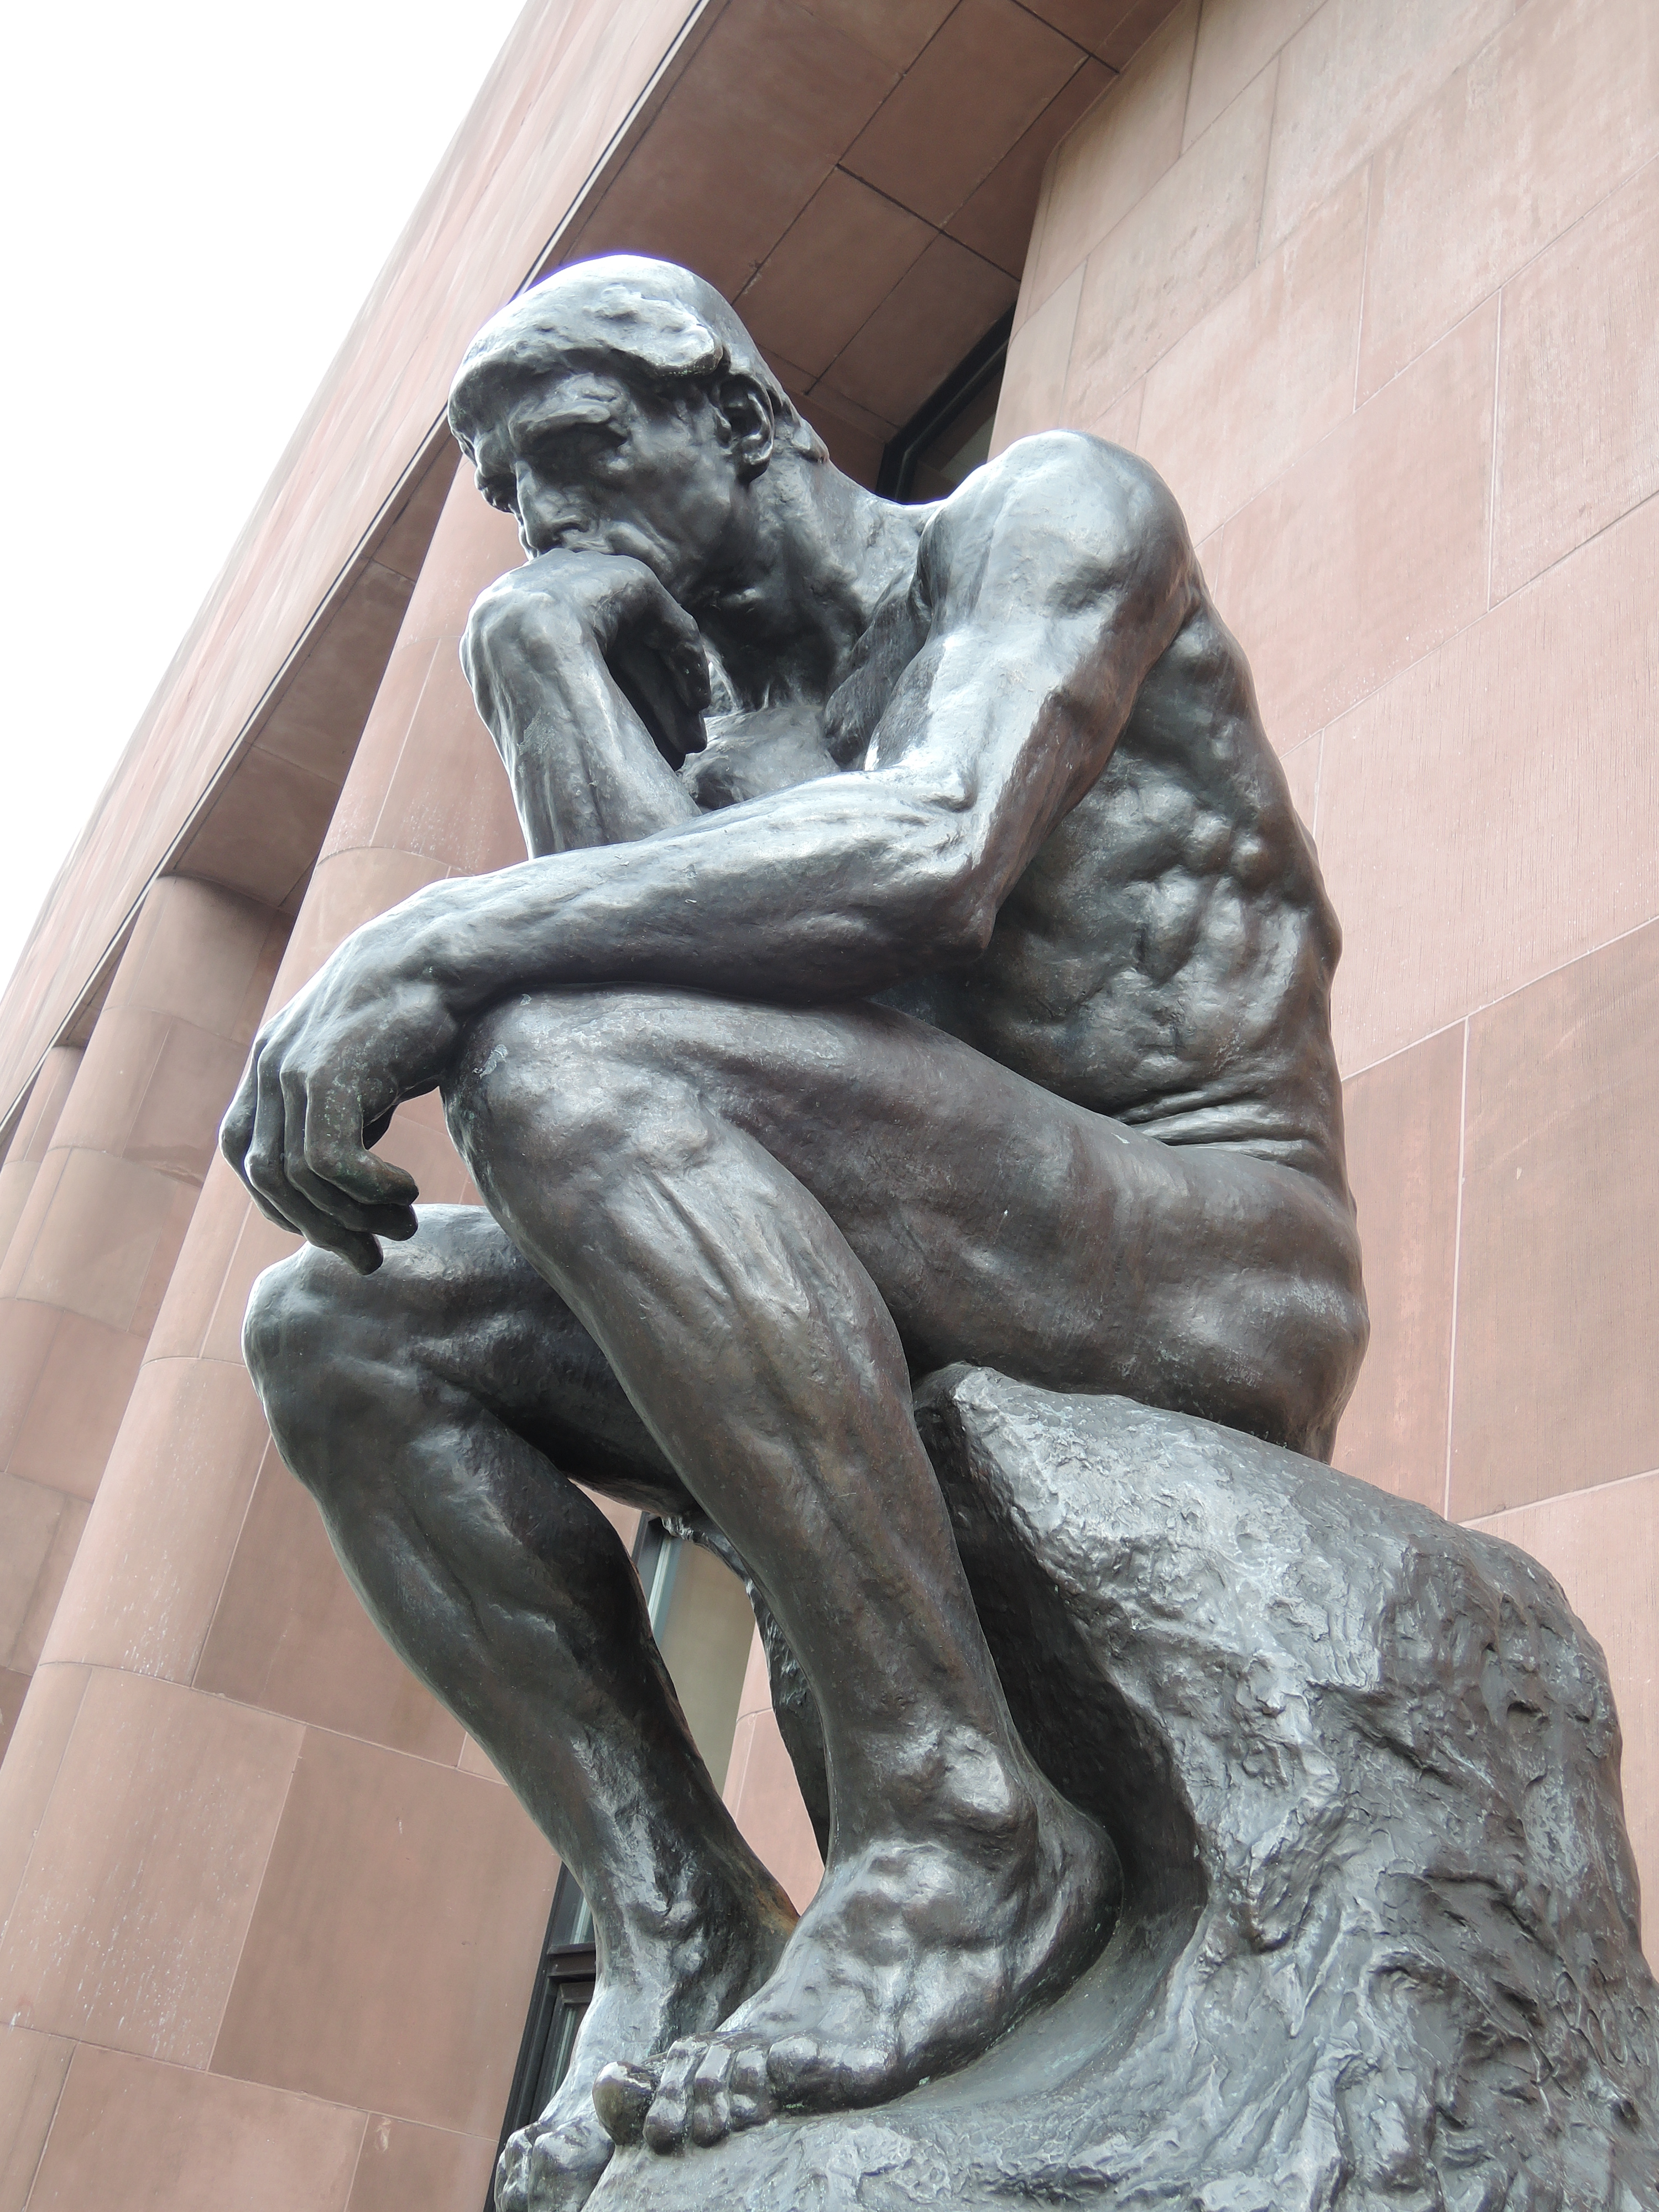
\includegraphics[width=0.12\textwidth]{images/thinker.jpeg}};

            % Small matrix
            \AnimateNode{4}{draw=none, inner sep=0pt} (program) at ($(robot) + (3.5cm, 0.5cm)$) {\scriptsize 1 0 1 0 0 1};
            \AnimateNode{4}{draw=none, inner sep=0pt} (program2) at ($(robot) + (3.5cm, 0.2cm)$) {\scriptsize 1 0 1 0 1 0};
            \AnimateNode{4}{draw=none, inner sep=0pt} (program3) at ($(robot) + (3.5cm, -0.1cm)$) {\scriptsize 0 0 1 1 0 0};
            \AnimateNode{4}{draw=none, inner sep=0pt} (program4) at ($(robot) + (3.5cm, -0.4cm)$) {\scriptsize 1 0 1 1 1 0};

            % Graph edits
            \AnimateNode{4}{circle, inner sep=3pt, fill=themefont} (n1) at
                ($(program) + (2.9cm, 0cm)$) {};
            \AnimateNode{4}{circle, inner sep=3pt, fill=themefont} (n2) at
                ($(n1) + (1cm, -0.33cm)$) {};
            \AnimateNode{4}{circle, inner sep=3pt, fill=themestrong} (n3) at
                ($(n1) + (1.5cm, -1cm)$) {};
            \AnimateNode{4}{circle, inner sep=3pt, fill=themeaccent} (n4) at
                ($(n1) + (0cm, -0.65cm)$) {};
            \AnimateNode{4}{circle, inner sep=3pt, fill=themefont} (n5) at
                ($(n1) + (0.45cm, -1cm)$) {};
            \AnimateNode{4}{circle, inner sep=3pt, fill=themetitle} (n6) at
                ($(n1) + (1.25cm, 0.25cm)$) {};

            \AnimateDraw{4}{-, themefont} (n1) -- (n2);
            \AnimateDraw{4}{-, themefont} (n1) -- (n4);
            \AnimateDraw{4}{-, themefont} (n2) -- (n3);
            \AnimateDraw{4}{-, themefont} (n4) -- (n5);
            \AnimateDraw{4}{-, themefont} (n2) -- (n6);

            % text labels
            \AnimateNode{4}{draw=none} (dlabel) at ($(dinosaur) + (0cm, -0.9cm)$)
                {\footnotesize{1. Fuzzer stuck}};

            \AnimateNode{4}{draw=none} (rlabel) at ($(robot) + (0cm, -1.6cm)$)
                {\footnotesize{2. Ask large language friend}};

            \AnimateNode{4}{draw=none} (plabel) at ($(program) + (0cm, -1.5cm)$)
                {\footnotesize{3. Gather context}};

            \AnimateNode{4}{draw=none} (glabel) at ($(n1) + (0.75cm, -1.5cm)$)
                {\footnotesize{4. Make graph edits}};

            % Accented arrows
            \AnimateDraw{4}{->, themeaccent} (dinosaur.east) --
                ($(robot.west) + (-0.2cm, 0cm)$);
            \AnimateDraw{4}{->, themeaccent}
                ($(dinosaur.east) + (4.0cm, 0cm)$)  --
                ($(dinosaur.east) + (5.4cm, 0cm)$);
            \AnimateDraw{4}{->, themeaccent}
                ($(dinosaur.east) + (7.35cm, 0cm)$)  --
                ($(dinosaur.east) + (8.75cm, 0cm)$);
        \end{tikzpicture}

        \AnimateOnly{5}
        {
            \vspace{-1.33cm}
            \begin{small}
                \inputminted[style=gruvbox-dark]{python}{code/harness_small.py}
            \end{small}
        }
        \AnimateOnly{6}
        {
            \centering
            \vspace{-1cm}
            \begin{tabular}{c|c|c}
                Model & Size & Correctness (N = 100) \\
                \hline
                Granite 4-1:30b & 17G & 49\% \\
                Deepseek-r1:14b & 9G & 4\% \\
                qwen-3.8 & 17G & 90\% \\
                Sonnet 4.6 & cloud & 99\% \\
            \end{tabular}
            \vspace{-1.4cm}
        }

        % Offsets and things to mitigate jitter
        \AnimateOnly{2}{\vspace{-2.75cm}}
        \AnimateOnly{3}{\vspace{-3cm}}
        \AnimateOnly{5}{\vspace{-2cm}}
        \AnimateOnly{7}{
            \vspace{-1.15cm}
            \begin{center}
                \textit{Vibe fuzzing offers a robust, cost-effective means for long-term testing and VR.}
            \end{center}
        }
    }{%
        \vspace{0.5cm}
        Vibe fuzzing offers a robust, cost-effective means for long-term testing and VR.
    }
\end{frame}

\iftoggle{ANIMATIONS}{%
    % Reset dino
    \setbeamertemplate{headline}{
        \iftoggle{DINOSAUR}{%
            \begin{tikzpicture}[remember picture, overlay]
                \node[draw=none, inner sep=0pt] (dino) at ($(current page.north east) + (-1cm, -1cm)$)
                    {
\includegraphics[width=0.055\textwidth]{images/dino.png}};
            \end{tikzpicture}
        }{}
    }
}{}

\begin{frame}{Thank yous!}
    \begin{center}
        \begin{large}
            \color{themeaccent}
            Dustin Heywood \\
            Valentina Palmiotti \\

            \vspace{1cm}
            OAIC Organization Crew \\
        \end{large}
        \vspace{0.75cm}
        vf3 release w/ benchmarks coming November 2026 (@\_dinolover38 for updates)
    \end{center}
    \vspace{-.25cm}
\end{frame}
